\section{Introduction}

The parallel programming languages, e.g., OpenCL, are based on BSP (Bulk Synchronous Parallel) model and are widely adopted by GPUs, which features a massive number of cores for the computation task. 
Due to the fact that FPGA is embarrassingly parallel, it is a natural attempt to use the existing parallel programming languages to program FPGA. For instance, Intel has launched an end-to-end OpenCL SDK to program FPGAs~\cite{altera_optimization} such that the complexity from direct hardware programming (e.g., Verilog) is abstracted away. OpenCL delivers increased programmability and lower learning curve with respect to RTL. Accordingly, plenty of research work~\cite{flexcl_tc18, opencl_compiler_ERSA12, fpga_opencl_model_hpca16} are aim at optimizing the \emph{conventional OpenCL} kernels on FPGAs, where the conventional OpenCL kernel is the NDRange kernel which employs a multi-thread approach to accelerate the computing task. 
%The optimization process is vital to achieve good performance on FPGAs, since the performance difference between proper and improper optimizations can be significant. For example, [X] shows that the optimal combination of optimization methods can provide two orders of magnitude better performance than the baseline without optimization. 

%\jgl{I think an interesting motivation for this work can be achieving performance portability across different types of accelerators (i.e., GPU to FPGA). In this regard, a paper to cite is \cite{chang2017collaborative}.}

%\jgl{Somewhere in the introduction, it is necessary to talk about the characteristics of the GPU OpenCL codes that are going to be ported to FPGA in this work. In Chai \cite{gomez2017chai}, there are benchmarks that use inter-kernel communication (e.g., CEDD) and multi-pass schemes (e.g., BFS, SSSP). These two are typical techniques in GPU programming. In Chai, there is also extensive use of atomic operations. In the past, GPU programmers avoided atomic operations \cite{nasre2013} because they had high overhead. However, in recent GPU generations (e.g., NVIDIA Kepler, Maxwell, Pascal) the hardware has greatly improved. They provide improved programmability that GPU programmers nowadays leverage.}

Despite the preliminary success from directly adopting conventional OpenCL programs on FPGAs, we still identify a significant gap from achieving near-optimal performance on FPGAs due to the factor that the conventional OpenCL kernel cannot always represent FPGA resources in an efficient way. In particular, it is not able to fully utilize two FPGA-aware features, referred as go-beyond OpenCL features for FPGAs. %We discuss the features in two dimensions. %the architecture of FPGAs is significantly different from that of GPUs  \jgl{Any related work that has compared the performance of optimized RTL with OpenCL?}

\vspace{0.3em}
\noindent
{\bf F1: Single Work-Item (SWI) Kernel. }Intel OpenCL SDK provides a new programming model for FPGAs: \emph{single work-item kernel}. It relies on the off-line compiler to explore the pipelined parallelism at the compilation time. Therefore, it only contains only one work item to do the computation, indicating significantly different from data-parallel programming model of conventional OpenCL kernel. %The single work-item execution pattern more closely matches the traditional deep-pipeline approach of programming FPGAs.
%First, the external memory bandwidth on FPGAs is critically less than that on GPUs. This means that memory bandwidth on FPGAs can much easier become the performance bottleneck.  

\vspace{0.3em}
\noindent
{\bf F2: Direct Kernel-to-Kernel Communication. }The communication between two kernels can be done via a FIFO (i.e., OpenCL channel) on FPGAs, not via memory subsystem like GPUs. It can potentially reduce memory traffic and achieve more parallelism by concurrently executing multiple OpenCL kernels on FPGAs. 
%OpenCL programs are originally designed for GPUs
\vspace{0.3em}

%Actually, several research work~\cite{partition_fpl15, gzip_iwocl14} have already employed the above two techniques to significantly accelerate a broad range of OpenCL applications. For instance, the performance of database partitioning~\cite{partition_fpl15} is improved by 10.7 times thanks to the OpenCL channel, indicating a great potential of go-beyond kernel on FPGAs. Together with the optimization methods from conventional OpenCL kernel, a huge design space needs to be explored to determine the optimal (or near-optimal) optimization combination on FPGAs. 
Unfortunately, there is no comprehensive study to guide the OpenCL programmer how to optimize the OpenCL kernels on FPGAs in the context of go-beyond OpenCL features, so the burden of choosing the right OpenCL optimization methods (e.g., go-beyond OpenCL features) still falls on OpenCL programmers without any rule-of-thumb guidelines. %In this paper, we try to bridge the gap between application and OpenCL execution pattern. In particular, 
%a comprehensive study, which can  is still lacking.
Therefore, we ask the following question: 

\vspace{0.4em}
%{\em Can we narrow the gap between conventional OpenCL programmer and performance potential of FPGAs?}
{\em Can we explicitly determine whether to use go-beyond OpenCL or not for the conventional OpenCL programmer?}
\vspace{0.4em}
%\vspace{-0.2em}
%\begin{center}
%	{\em Can we bridge the gap between conventional OpenCL programmer and high performance on FPGAs?}
%\end{center}
%\vspace{-0.2em}

%As a start, we try to bridge the gap between OpenCL patterns and execution models.
In this paper, we make the following contributions to answer the question by connecting three typical OpenCL patterns and four high-level execution models. As such, the OpenCL programmer can directly decide whether to use go-beyond OpenCL or not (in terms of execution model), based on three well known OpenCL patterns. %The key idea is that the execution model is determined by .the conventional OpenCL programmer are familiar with these OpenCL patterns.  (aware of go-beyond OpenCL features)

%\jgl{To me, the most significant contribution of this work can be providing some guidelines on how to transform optimized GPU OpenCL code into optimized FPGA OpenCL.} 

\vspace{0.4em}
\noindent
{\bf C1: Three Typical OpenCL Patterns on FPGAs (Section~\ref{sec_patterns}). }We identify three typical patterns from OpenCL kernels on GPUs: atomic operation, multi-pass scheme and kernel-to-kernel communication, which are worth to be heavily revisited on FPGAs, since their performance can be significantly improved with the help of go-beyond-OpenCL features enabled by FPGAs. Since these patterns are well understood by the conventional OpenCL programmers, they can serve as a really nice starting point from OpenCL side. %easily identify the potentials of their original OpenCL program which maps onto FPGAs. %Besides,  can easily understand these patterns. %the architecture of FPGAs is significantly different from that of GPUs. In particular, 

\vspace{0.4em}
\noindent
{\bf C2: Four High-level Execution Models on FPGAs (Section~\ref{sec_execution_models}). }We identify four high-level OpenCL execution models: NDRange, SWI, NDRange+Channel and SWI+Channel, which are allowed by the OpenCL SDK for FPGAs. Choosing the right execution model actually determines the performance upper bound of the further optimization process. Figure~\ref{fig_intro_performance_difference} shows that the performance ratio of the most suitable to the most unsuitable execution models, where the best optimization combination has already been employed for each execution model. The exact execution models used by each application are not important here. We refer the interested reader to Section~\ref{sec_experiment} for more details. We can observe that the performance difference can achieve three orders of magnitude. It shows the importance of choosing the right execution model, which should serve as the first and the most important step to determine for optimizing OpenCL kernel on FPGAs. %serves as the main guidelines on how to optimize the OpenCL program on FPGAs. 
%We also generally compare the characteristics of four execution models, which are aware of the advanced features of go-beyond OpenCL kernel. 
\begin{figure}
	\centering
	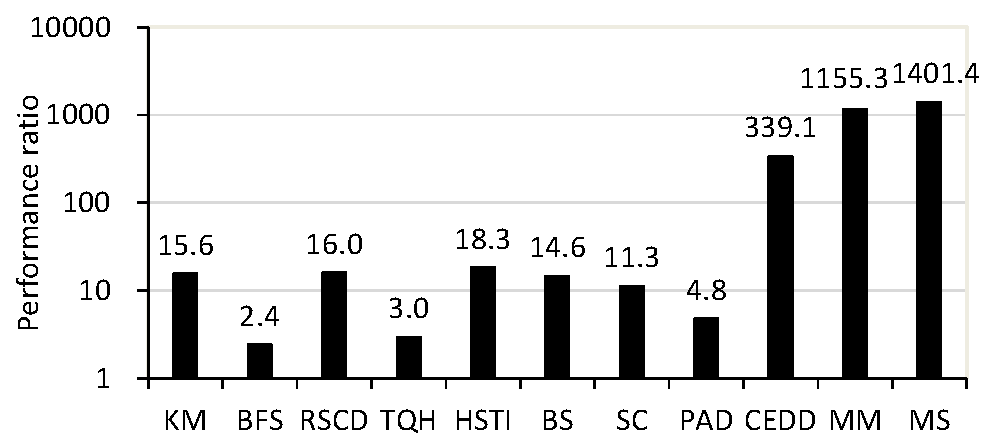
\includegraphics[width=0.45\textwidth]{performance_ratio.pdf}
	\vspace{-2.0ex}
	\caption{Performance difference between the most suitable and unsuitable execution models.}% We focus on the FPGA and main memory.
	\vspace{-2ex}
	\label{fig_intro_performance_difference}
\end{figure} 


%\vspace{0.4em}
%\noindent
%{\bf C3. Bridge the Gap between Patterns and Execution Models. }We identify three OpenCL patterns which show great opportunity to...
%
%Bridge the gap between OpenCL programmer and FPGAs. In particular, we provide a OpenCL-programmer-understandable approach 
\vspace{0.4em}
\noindent
{\bf C3. Intensive Experiment to Verify the Connection (Sections~\ref{sec_bridge_gap}, \ref{sec_experiment}). }We implement and optimize 11 OpenCL applications on a Terasic\textquoteright s DE5A-Net Arria 10 FPGA board. We make our best effort\footnote{Based on our five years' experience on OpenCL-based FPGAs, we are pretty sure that our implementation have typically reached the near-optimal performance for each execution model. We will make all the related source code open-sourced. } to explore optimization combinations for all the four execution models for each OpenCL application. Based on the experimental result, we can observe that the real execution model (which has the best performance) can match the predicted execution model, which is determined by three OpenCL patterns. %we can make two observations. First, different high-level execution model leads to up to three orders of magnitude performance difference. Second, we identify a obvious connection between three proposed OpenCL channels and four high-level execution models. 
%We try to show the potential of different execution models by quantitatively analyze the performance difference. , each of which contains multiple optimization combinations,
%\footnote{For few applications, it is impossible to implement few execution models.}

\vspace{0.7em}
%This paper is orthogonal to the existing literature.
This paper can serve as a complementary guideline for the existing optimization efforts~\cite{flexcl_tc18, opencl_compiler_ERSA12, fpga_opencl_model_hpca16}. Besides, we argue that determining the execution model should be considered as the first step to decide, as it determines the potential of further optimization combinations can reach. 

\vspace{0.5em}
\noindent
{\bf Future Directions. } 
To the best of our knowledge, this paper is the first attempt to guide the conventional OpenCL programmer to leverage go-beyond OpenCL or not, and we believe it opens a few exciting research directions so that it will attract more and more people to devote to FPGA acceleration. One future direction is to provide an end-to-end performance analytical model to predict the performance of go-beyond OpenCL kernels. Until now, the literature only cover the analytical model for the NDRange kernel~\cite{fpga_opencl_model_hpca16, flexcl_tc18}. 
Another interesting future direction is to design an automatic optimization process for each execution model with the help of performance analytical model. As such, more and more OpenCL programmer without any FPGA background can take advantage of computing power of FPGAs. 

\vspace{0.7em}
\noindent
{\bf Limitations. }This work has two limitations. First, we manually try plenty of optimization combinations for each execution model. Second, for a few applications, we cannot successfully implement all the four execution models. In particular, the result is not correct. %Based on our five years' experience on OpenCL-based FPGAs, we are pretty sure that our implementation have typically reached the near-optimal performance for each execution model. 

%Deciding the right execution pattern is rule-of-thumb to determine the performance of  




%Third, where communication among cores is done via memory subsystem, e.g., external memory. In particular, each core writes its result to the memory subsystem and then synchronize to make sure the core can see the latest result from other cores. The underlying reason is that no communication channel exists between any two cores. This execution pattern works well on GPUs due to its powerful memory subsystem



%in this paper, we explore the design space of accelerating OpenCL programs on FPGAs, especially focusing on the go-beyond OpenCL part. In particular, 

%Towards a comprehensive 

